\documentclass[a4paper,11pt]{report}
\usepackage[T1]{fontenc}
\usepackage[utf8]{inputenc}
\usepackage{lmodern,url}
\usepackage{graphicx}
\usepackage{hyperref}
\usepackage{pslatex}
\usepackage{listings}
\usepackage{textcomp}
\usepackage{float}
\usepackage[paper=a4paper,headheight=0pt,left=4cm,top=3cm,right=3cm,bottom=3cm]{geometry}
\usepackage{titling}
\usepackage{pdfpages}
\usepackage{booktabs}
\usepackage[version=4]{mhchem}
\usepackage{isotope}
\usepackage{datetime2}
\usepackage{rotating}
\usepackage{pdflscape}
\usepackage{subfigure}
\usepackage[version=4]{mhchem}
\usepackage{isotope}
\DTMsetdatestyle{ddmmyyyy}
\DTMsetup{datesep=--}
\newcommand{\subtitle}[1]{%
  \posttitle{%
    \par\end{center}
    \begin{center}\large#1\end{center}
    \vskip0.5em}%
}
\newcommand{\ra}[1]{\renewcommand{\arraystretch}{#1}}
\newcommand{\addChapter}[1]{\phantomsection \addcontentsline{toc}{chapter}{#1}}
% Tambahkan berkas PDF ke dalam laporan dan gunakan style laporan  
% terhadap berkas ini. 
\newcommand{\inpdf}[1]{
	\includepdf[pages=-,pagecommand={\thispagestyle{fancy}}]{#1.pdf}}
% 
% Tambahkan berkas PDF ke dalam laporan. 
\newcommand{\putpdf}[1]{\includepdf[pages=-]{#1.pdf}}
\renewcommand*\descriptionlabel[1]{\hspace\leftmargin$#1$}
% 
%
% Hyphenation untuk Indonesia 
%
% @author  Andreas Febrian
% @version 1.00
% 
% Tambahkan cara pemenggalan kata-kata yang salah dipenggal secara otomatis 
% oleh LaTeX. Jika kata tersebut dapat dipenggal dengan benar, maka tidak 
% perlu ditambahkan dalam berkas ini. Tanda pemenggalan kata menggunakan 
% tanda '-'; contoh:
% menarik
%   --> pemenggalan: me-na-rik
%

\hyphenation{
    % alphabhet A
    a-na-li-sa a-tur 
    a-pli-ka-si 
    % alphabhet B
    ba-ngun-an 
    be-be-ra-pa 
    ber-ge-rak
    ber-ke-lan-jut-an 
    ber-pe-nga-ruh 
    ber-o-pe-ra-si
    % alphabhet C
    ca-ri cri-ti-cal
    % alphabhet D
    di-sim-pan di-pim-pin de-ngan da-e-rah di-ba-ngun da-pat di-nya-ta-kan 
    di-sim-bol-kan di-pi-lih di-li-hat de-fi-ni-si di-de-fi-ni-si-kan
    di-mo-del-kan di-te-rap-kan
    di-ha-rap-kan
    di-e-va-lu-a-si
    di-su-sun
    di-sa-ji-kan
    % alphabhet E
    e-ner-gi eks-klu-sif
    % alphabhet F
    fa-si-li-tas
    % alphabhet G
    ga-bung-an ge-rak
    % alphabhet H
    ha-lang-an
    % alphabhet I
    % alphabhet J
    % alphabhet K
    ke-hi-lang-an
    ku-ning 
    kua-li-tas ka-me-ra ke-mung-kin-an ke-se-pa-ham-an
    % alphabhet L
    ling-kung-an
    % alphabhet M
    me-ne-ngah
    meng-a-tas-i me-mung-kin-kan me-nge-na-i me-ngi-rim-kan 
    meng-u-bah meng-a-dap-ta-si me-nya-ta-kan mo-di-fi-ka-si
    meng-a-tur
    meng-a-la-mi
    meng-u-kur
    me-re-pre-sen-ta-si-kan
    men-da-pat-kan
    % alphabhet N
    nya-ta non-eks-klu-sif nu-klir
    % alphabhet O
    o-pe-ra-si
    % alphabhet P
	pe-nye-rap-an 
	pe-ngon-trol
    pe-mo-del-an
    pe-ran  pe-ran-an-nya
    pem-ba-ngun-an pre-si-den pe-me-rin-tah prio-ri-tas peng-am-bil-an 
    peng-ga-bung-an pe-nga-was-an pe-ngem-bang-an 
    pe-nga-ruh pa-ra-lel-is-me per-hi-tung-an per-ma-sa-lah-an 
    pen-ca-ri-an peng-struk-tur-an
    per-siap-an pa-ra-me-ter
    pa-sang-an
    % alphabhet Q
    % alphabhet R
    ran-cang-an
    % alphabhet S
    si-mu-la-si sa-ngat
    se-dang-kan sa-tu-an
    % alphabhet T
    te-ngah
    ter-da-pat
    % alphabhet U
    % alphabhet V
    % alphabhet W
    % alphabhet X
    % alphabhet Y
    % alphabhet Z
    % special
}

\definecolor{amber}{rgb}{0.96, 0.51, 0.13}
\definecolor{biruMuda}{rgb}{0.45, 0.62, 0.78}

\renewcommand{\contentsname}{Daftar Isi}
\renewcommand{\chaptername}{BAB}
\renewcommand{\bibname}{Daftar Referensi}
\renewcommand{\listfigurename}{Daftar Gambar}
\renewcommand\lstlistlistingname{Daftar Program}
\renewcommand{\figurename}{Gambar}
\renewcommand{\tablename}{Tabel}
%\title{Lampiran II}
%\title{Kajian Komputasi Dinamika Fluida berbasis OpenFOAM}
%\author{Arya Adhyaksa Waskita}
%\date{January 31, 2017}
\begin{document}
\begin{titlepage}

\newcommand{\HRule}{\rule{\linewidth}{0.5mm}} % Defines a new command for the horizontal lines, change thickness here

\center % Center everything on the page


%----------------------------------------------------------------------------------------
%	LOGO SECTION
%----------------------------------------------------------------------------------------


\includegraphics[scale=.25]{pics/logo.png}\\[1cm] % Include a department/university logo - this will require the graphicx package

%----------------------------------------------------------------------------------------
%	TITLE SECTION
%----------------------------------------------------------------------------------------

\HRule \\[0.4cm]
{ \huge \bfseries Dokumen Pengembangan TRIAMIX \\ (TRIso \textit{Analysis Code} coupled with THERMIX capabilities)}\\[0.4cm] % Title of your document
\HRule \\[1.5cm]

%----------------------------------------------------------------------------------------
%	HEADING SECTIONS
%----------------------------------------------------------------------------------------
%\textsc{Sub Bidang Termohidrolika}\\[0.25cm] % Minor heading such as course title
\textsc{Laboratorium Komputasi}\\[0.25cm] % Major heading such as course name
\textsc{\Large Pusat Teknologi dan Keselamatan Reaktor Nuklir}\\[1.5cm] % Name of your university/college

 
%----------------------------------------------------------------------------------------
%	AUTHOR SECTION
%----------------------------------------------------------------------------------------

\begin{minipage}{0.4\textwidth}
\begin{flushleft} \large
\emph{Disusun oleh:}\\
Arya Adhyaksa Waskita
\end{flushleft}
\end{minipage}
~
\begin{minipage}{0.4\textwidth}
\begin{flushright} \large
\emph{Supervisor:} \\
Dr. Eng. Topan Setiadipura
\end{flushright}
\end{minipage}\\[4cm]

% If you don't want a supervisor, uncomment the two lines below and remove the section above
%\Large \emph{Author:}\\
%John \textsc{Smith}\\[3cm] % Your name

%----------------------------------------------------------------------------------------
%	DATE SECTION
%----------------------------------------------------------------------------------------

{\large \today}\\[3cm] % Date, change the \today to a set date if you want to be precise
%{\large 31 Juli 2017}\\[3cm] % Date, change the \today to a set date if you want to be precise
 
%----------------------------------------------------------------------------------------

\vfill % Fill the rest of the page with whitespace

\end{titlepage}

%\tableofcontents

\pagenumbering{roman}
%\maketitle
\clearpage
\setcounter{page}{2}
\addChapter{Daftar Gambar}
\tableofcontents
%\clearpage
\listoffigures
\addChapter{Daftar Program}
\lstlistoflistings
%\clearpage
\pagenumbering{arabic}

\chapter{Pendahuluan}
Analisis keselamatan reaktor nuklir melibatkan sejumlah aspek seperti diperlihatkan pada \figurename~\ref{fig:aspek}. Setelah upaya melakukan rekayasa balik terhadap PANAMA \cite{report1,VERFONDERN201484} untuk aspek kinerja bahan bakar \cite{triac1}, dipandang perlu untuk melanjutkan analisis keselamatan di aspek \textit{thermal hydraulics}.

\begin{figure}[h!]
  \begin{center}
    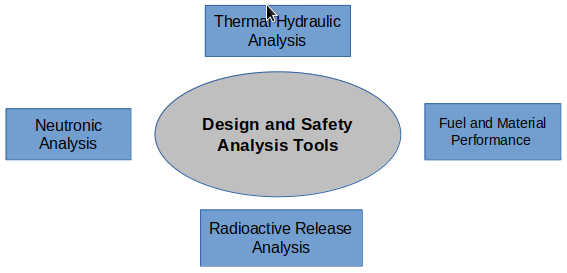
\includegraphics[scale=.5]{pics/tools.png}
    \caption{Aspek keselamatan reaktor nuklir}
    \label{fig:aspek}
  \end{center}
\end{figure}

Kode komputer THERMIX \cite{vsop1,vsop2} sebagai salah satu kode baku dalam analisis keselamatan reaktor di aspek termal yang turut menghantarkan Jerman sebagai \textit{center of excellent} pada penelitian tersebut. Dari THERMIX, sejarah irradiasi dan kecelakaan yang dialamai partikel triso dapat disimulasikan.

Karenanya, perangkat lunak akan dikembangkan berdasarkan data referensi dan dokumentasi  \textbf{\cite{vsop1,vsop2}}. Hasil rekayasa balik akan berupa prototipe kode komputer/perangkat lunak yang terintegrasi dengan modul analisis keselamatan bahan bakar berbasis partikel triso \cite{triac1} dan analisis ketidakpastian \cite{lhs}.

\chapter{Struktur Program}

\section{Diagram konteks}
Sistem yang akan dikembangkan memiliki diagram konteks level 0 seperti pada \figurename~\ref{fig:level0}. Triamix akan menerima masukan berupa distribusi rapat daya dan menghasilkan distribusi temperatur. Distribusi temperatur tersebut selanjutnya akan menjadi masukan bagi TRIAC-BATAN yang sebelumnya dikembangkan \cite{triac1}.

\begin{figure}[h!]
  \begin{center}
    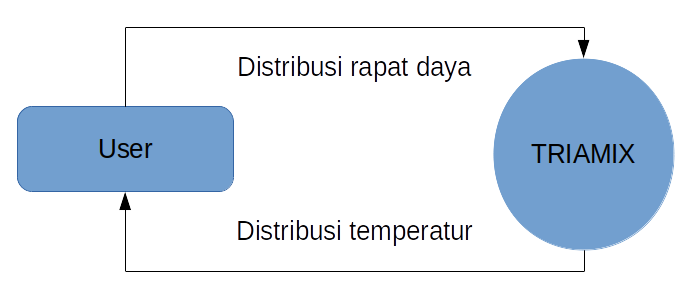
\includegraphics[scale=.4]{pics/contextLevel0.png}
    \caption{Konteks level 0 dari sistem Triamix}
    \label{fig:level0}
  \end{center}
\end{figure}

\section{Kebutuhan fungsi}
Tahapan selanjutnya adalah membuka struktur program dan melihat keterkaitan antar fungsi yang terdapat di kode komputer THERMIX. Terdapat 4 program, masing-masing \texttt{THERMIX1.FOR} - \texttt{THERMIX4.FOR}. Subrutin dan fungsi pada masing program tersebut disajikan pada \tablename~\ref{tab:the1} - \tablename~\ref{tab:the4}. Deskripsi yang disajikan merupakan translasi bebas dari Bahasa Jerman menggunakan \href{https://translate.google.com/}{google translate}.

\begin{table}[h!]
  \caption{Daftar fungsi dan subrutin dalam program \texttt{THERMIX1.FOR}}
  \label{tab:the1}

  \begin{center}
    \begin{tabular}{p{3cm}|p{10cm}}
    \toprule
       Fungsi / Subrutin & Deskripsi\\ \midrule
       ABEND & Membuat penanganan kesalahan \\
       BILD & Lembar penciptaan buatan dan halaman akhir \\
       BUBIL & Perhitungan sumber panas konvektif saat ini dan kompensasi komposisi ini. Hanya aktif jika sumber panas dibuat dengan $\alpha * f$ dan \texttt{TFLU} \\
       CALT & Hitung suhu pada kondisi tunak \\
       CALT1 & Menghitung suhu suhu padat yang homogen \\
       CALT2 & Menghitung suhu padat heterous (temperatur zona bola) solusi TRISSIAG dari sistem persamaan penghapusan matriks (GAUSS) \\
       CALT2H & Menghitung suhu padat heterous (temperatur zona bola) solusi sistem persamaan TRIDIAG matriks penghapusan (GAUSS) \\
       CALTA & Menghitung temperatur padat heterous (\textit{stationary billing}) solusi sistem persamaan sebagai SR CALT2 (eliminasi matriks) \\
       CALTAH & Menghitung temperatur padat heterous (\textit{stationary billing}) solusi sistem persamaan sebagai SR CALT2 (eliminasi matriks) \\
       EXPLIZ & Perhitungan eksplisit ke fungsi panas \\
       MAITHX & Program utama THERMIX, 50x80 tingkat perubahan \\
       STEUER & Menetapkan suhu tengah, menciptakan plot waktu, temperatur corr. rangkaian dalam arah y \\ 
       WTSTEU & Kendali penghapusan kinerja di pertukaran panas \\
       \bottomrule
    \end{tabular}
  \end{center}
\end{table}

\begin{table}[h!]
  \caption{Daftar fungsi dan subrutin dalam program \texttt{THERMIX2.FOR}}
  \label{tab:the2}

  \begin{center}
    \begin{tabular}{p{3cm}|p{10cm}} \toprule
    Fungsi / Subrutin & Deskripsi\\ \midrule
    DDF1 & Tidak tersedia penjelasan \\
    CALT3 & Perhitungan suhu pada heterous (temperatur zona bola) solusi sistem persamaan Gauss-Siedel. Hati-hati menggunakan $\rightarrow$ \texttt{kapasitas panas*WK} APH, tidak bekerja untuk \textit{flash ball} \\
    EINL1 & Program \texttt{READOUT} untuk bagian program \texttt{HEATER} \\
    GFIT & Perhitungan perubahan akurasi panas irradiasi \\
    GRPR & Penetapan \texttt{GR*PR} untuk cetakan konveksi bebas, \texttt{P} harus disediakan \\
    INTEST & Aktif dalam IFTEST=1 $\rightarrow$ angka minimum untuk uji masukan \\
    IPLOG & Interpolasi logaritmik pada nilai konstan melampaui rentang definisi \\
    ISOPLT & Plot iso-linear \\
    ITPL & Interpolasi linear \\
    KONST1 & Perhitungan kemampuan pemanasan dan fungsi geometri untuk \textit{shelves} \\
    KOPFB & Program \textit{coupling} untuk suhu dan umpan balik XENON \\
    KUEHLK & Tidak tersedia penjelasan\\
    MARK & Tanda batas komposisi dari luaran grid besar \\
    MIMAX & Menentukan minimum dan maksimum ruang grid terhubung \\
    ORDNE1 & Tidak tersedia penjelasan \\
    ORDNE2 & Pilih dari jumlah total 3 cm dukungan terbesar \\
    PDFELD & Masalah besar yang dilakukan di sini, konsentrasi VSOP untuk release produk fisi \\
    PRAIZ & Tidak tersedia penjelasan \\
    PREIN & Pengendalian dan output sifat komposisi \\
    PRFELD & Edisi grid yang hebat \\
    PRINTT & Masalah grille kecil \\
    READRZ & Masukan grille aksial dan radial \\
    \bottomrule
    \end{tabular}
  \end{center}
\end{table}

\begin{table}[h!]
  \caption{Daftar fungsi dan subrutin dalam program \texttt{THERMIX3.FOR}}
  \label{tab:the3}
  \begin{center}
    \begin{tabular}{p{3cm}|p{10cm}} \toprule
    Fungsi / Subrutin & Deskripsi\\ \midrule
      LAGRAS & Interpolasi lagrange \\
      POWTHX & Menerima layanan VSOP + EVTL konsentrasi terhadap grid thermix \\
      PRTEIN & Tidak tersedia penjelasan \\
      REDUM & Perhitungan daya termal (lokasi, waktu) \\
      REDUN & Perhitungan kekuatan termal (lokasi, waktu) untuk OTTO \\
      REDUZ & Pengendalian perhitungan daya panas \\
      REFL & Mengatur Kondisi RIM adiabatis pada grid \\
      REIPO & Program interpolasi (ke transmisi grid) \\
      RUND & Tidak tersedia penjelasan \\
      SECURE & Membuat berkas untuk \textit{restart}\\
      SETBER & Tidak tersedia penjelasan \\
      SETD & Set dosis cepat \\
      SETE & Set kinerja daya dan konsentrasi \\
      SETF1 & Membaca grille thermix \\
      SETF2 & Membaca ketebalan zona inti \\
      SETK1 & Menempatkan grille thermix dengan komposisi \\
      SETSTR & Mengidentifikasi dan memeriksa kolom beam \\
      SETT & Konfigurasi suhu awal \\
      SETZT1 & Mengalihkan suhu awal yang diambil dengan bantuan grille\\
      VOLMAT & Volume matriks \texttt{VSOP-THERMIX*BIRGIT} \\
      \bottomrule
    \end{tabular}
  \end{center}
\end{table}

\begin{table}[h!]
  \caption{Daftar fungsi dan subrutin dalam program \texttt{THERMIX4.FOR}}
  \label{tab:the4}
  \begin{center}
    \begin{tabular}{p{3cm}|p{10cm}} \toprule
    Fungsi / Subrutin & Deskripsi\\ \midrule
    EINL2 & Program sub \textit{dummy} untuk masukan \texttt{KINEX} \\
    KINEX & Program sub \textit{dummy} faktor tanpa \texttt{KINEX} (sub rutin kosong) \\
    KOPREG & Program sub \textit{dummy} untuk akun tanpa pengendalian (sub rutin kosong) \\
    SUCHET & Mendefinisikan lokasi tugas het-grid dan pengendalian \texttt{IFBH} \\
    SUCHMI & Menetapkan panel kendali \texttt{IFBH} campuran \\
    SYMBOL & Menetapkan \texttt{IFBER} \\
    TFELD & Kendali perhitungan iteratif suhu padat \\
    TNEU & Terkait relaksasi \\
    TPROZ & Membuat temperatur-volume analisis untuk teras dan menghitung suhu bahan bakar mediumdan moderator (untuk daerah \texttt{HET}) \\
    VORKON & Unsur hitung quarter-flaechen \\
    WDUKON & Menghitung aksesibilitas panas \\
    WKAP & Menghitung kapasitas panas untuk setiap waktu, untuk zone \textit{mesh} dan bola \\  
    WKN & Memperhitungkan unsur dengan sumber panas konvektif \\
    WKPT & Menghitung $\rho * C$ untuk meteri yang berbeda untuk \ce{Al2O3} dan tidak tergantung pada temperatur \\
    WPKON & Menghitung sumber panas konvektif, kerapatan sumber dan volumen asosiasi \\
    XKORR & Tidak tersedia penjelasan \\
    XLAM & Menghitung aksesibilitas panas \\
    XLAM1 & Menghitung aksesibilitas panas anisotropis \\ 
    XLAMT & Menghitung konduktivitas panas \\
    XLAMT1 & Karakterisasi temperatur anisotropis dan termperatur resistan pada arah-Y \\
    ZKUGL & Menghitung jumlah \ce{Be} di mesin HET dan mesin campuran \\
      \bottomrule
    \end{tabular}
  \end{center}
\end{table}

Selain itu, terdapat juga terdapat juga fungsi/sub rutin yang didefinisikan pada program di luar \texttt{THERMIX}. \tablename~\ref{tab:anomali} menyajikan fungsi-fungsi tersebut.

\begin{table}[h!]
  \caption{Daftar fungsi dan subrutin dalam program \texttt{THERMIX4.FOR}}
  \label{tab:anomali}
  \begin{center}
    \begin{tabular}{p{2cm}|p{2.75cm}|p{3cm}|p{4.5cm}} \toprule
    Sub rutin & Dipanggil dari & Didefinisikan di & Keterangan \\ \midrule
    EINL & \texttt{THERMIX1.FOR} & \texttt{KONVEK1.FOR} & didefinisikan menggunakan \texttt{SUBROUTINE} \\
    FRIST & \texttt{THERMIX1.FOR} & \texttt{VSOP0.FOR} & didefinisikan menggunakan \texttt{SUBROUTINE} \\
    KONVEK & \texttt{THERMIX1.FOR} & \texttt{KONVEK1.FOR} & didefinisikan menggunakan \texttt{SUBROUTINE} \\
    WTSTE1 & \texttt{THERMIX1.FOR} & \texttt{THERMIX1.FOR} & dipanggil dengan \texttt{ENTRY}, tanpa definisi (kosong)\\
    NACHW & \texttt{THERMIX1.FOR} & \texttt{DECHEAT.FOR} & didefinisikan menggunakan \texttt{SUBROUTINE} \\
    DDF & \texttt{THERMIX1.FOR} & \texttt{THERMIX1.FOR} (dalam fungsi yang sama) & tidak ditemukan fungsi/sub rutin yang pernah menggunakannya \\
    VOLMA1 & \texttt{THERMIX3.FOR} & \texttt{THERMIX3.FOR}, sub rutin VOLMAT & dipanggil dengan \texttt{ENTRY}\\
    VOLMA2 & \texttt{THERMIX3.FOR} & \texttt{THERMIX3.FOR}, sub rutin VOLMAT & dipanggil dengan \texttt{ENTRY}\\
    FRIST & \texttt{THERMIX4.FOR} & \texttt{VSOP0.FOR} & didefinisikan menggunakan \texttt{SUBROUTINE} \\
      \bottomrule
    \end{tabular}
  \end{center}
\end{table}

Keterkaitan antar fungsi/sub rutin ditampilkan secara grafis disajikan pada \figurename~\ref{fig:maithx}. Penyajian tersebut menggunakan konvensi:
\begin{itemize}
  \item \textcolor{red}{merah} $\rightarrow$ terdefinisi di \texttt{THERMIX1.FOR}
  \item \textcolor{yellow}{kuning} $\rightarrow$ terdefinisi di \texttt{THERMIX2.FOR}
  \item \textcolor{green}{hijau} $\rightarrow$ terdefinisi di \texttt{THERMIX3.FOR}
  \item \textcolor{blue}{biru} $\rightarrow$ terdefinisi di \texttt{THERMIX4.FOR}
  \item \textcolor{biruMuda}{biru muda} $\rightarrow$ terdifinisi di program selain \texttt{THERMIX1.FOR} s/d \texttt{THERMIX4.FOR}
  \item bayangan \textcolor{amber}{oranye} $\rightarrow$ memiliki ketergantungan terhadap fungsi/sub rutin di bawahnya, fungsi/sub rutin tersebut dapat berada di \texttt{THERMIX1.FOR} s/d \texttt{THERMIX4.FOR} atau bahkan di luar keempat program tersebut.
  \item secara umum, panah menunjukkan ketergantungan yang setara antara fungsi/sub rutin di lapisan pertama dengan lapisan-lapisan di bawahnya. Seperti ditunjukkan pada \figurename~\ref{fig:maithx}, sub rutin \texttt{MAITHX} membawahi semua sub rutin di bawahnya secara langsung, kecuali \texttt{SETBER}, \texttt{ABEND} dan \texttt{BILD}.
\end{itemize}

\begin{figure}[h!]
  \begin{center}
    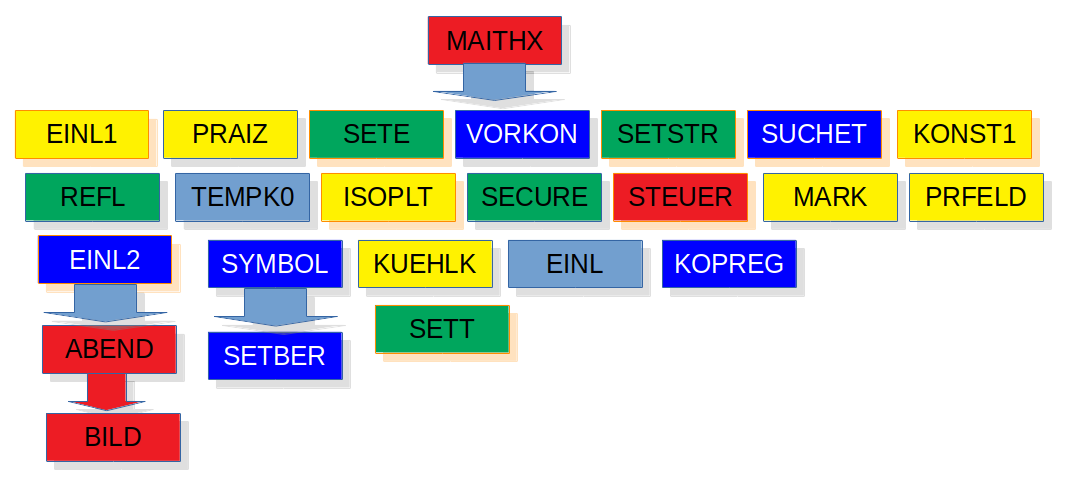
\includegraphics[scale=.5]{../maithx.png}
    \caption{Fungsi/sub rutin \texttt{MAITHX}, terbesar dari yang didefinisikan di \texttt{THERMIX}}
    \label{fig:maithx}
  \end{center}
\end{figure}

\vspace*{1cm}
Kemudian, sub rutin di bawah \texttt{MAITHX} yang membawahi sub rutin lain adalah:
\begin{enumerate}
  \item \texttt{EINL1} (\figurename~\ref{fig:einl1}),
  \item \texttt{SETE} (\figurename~\ref{fig:sete}),
  \item \texttt{SUCHET} (\figurename~\ref{fig:suchet}),
  \item \texttt{KONST1} (\figurename~\ref{fig:konst1}),
  \item \texttt{TFELD} (\figurename~\ref{fig:tfeld}),
  \item \texttt{ISOPLT} (\figurename~\ref{fig:isoplt}) dan
  \item \texttt{STEUER} (\figurename~\ref{fig:steuer}).
\end{enumerate}
        
\begin{figure}[h!]
  \begin{center}
    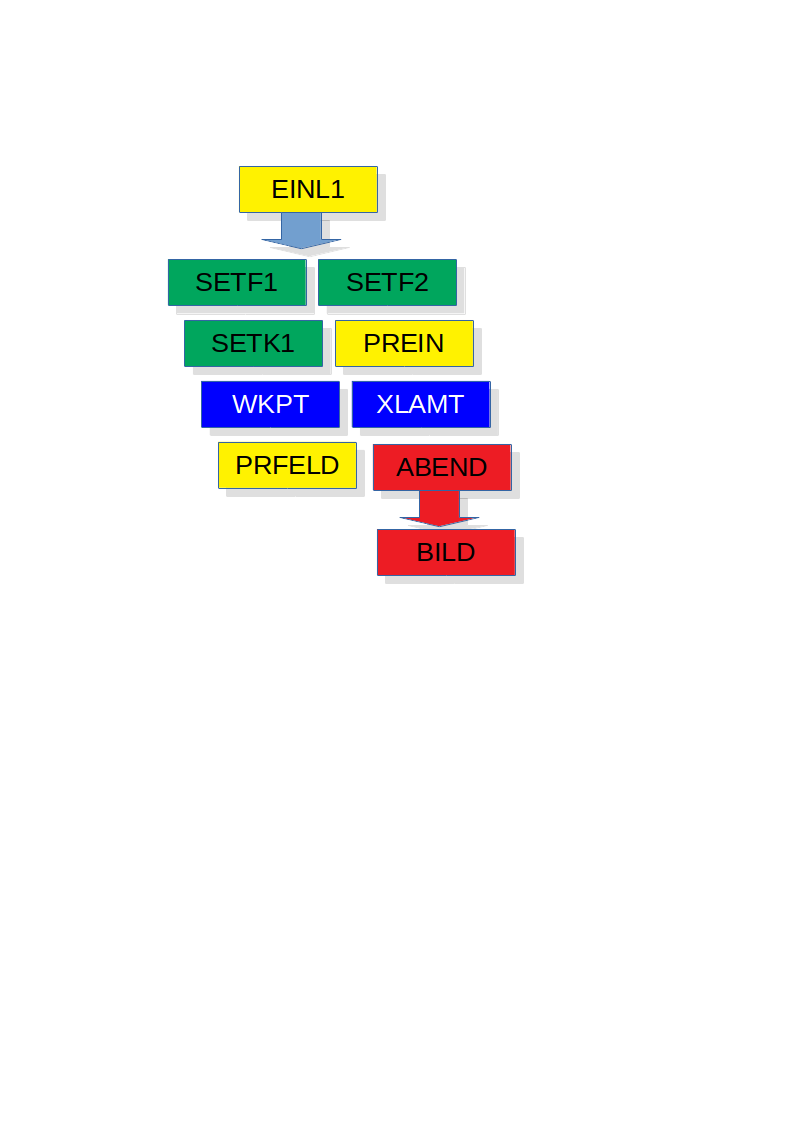
\includegraphics[scale=.5]{../einl1.png}
    \caption{Sub rutin \texttt{EINL1}}
    \label{fig:einl1}
  \end{center}
\end{figure}

\begin{figure}[h!]
  \begin{center}
    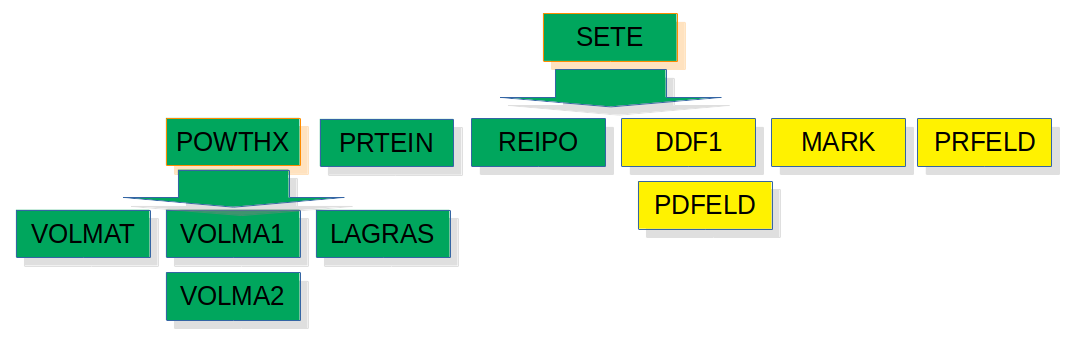
\includegraphics[scale=.5]{../sete.png}
    \caption{Sub rutin \texttt{SETE}}
    \label{fig:sete}
  \end{center}
\end{figure}

\begin{figure}[h!]
  \begin{center}
    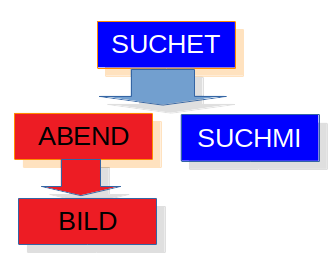
\includegraphics[scale=.5]{../suchet.png}
    \caption{Sub rutin \texttt{SUCHET}}
    \label{fig:suchet}
  \end{center}
\end{figure}

\begin{figure}[h!]
  \begin{center}
    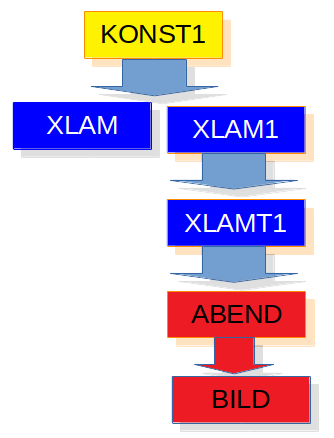
\includegraphics[scale=.5]{../konst1.png}
    \caption{Sub rutin \texttt{KONST1}}
    \label{fig:konst1}
  \end{center}
\end{figure}

\begin{figure}[h!]
  \begin{center}
    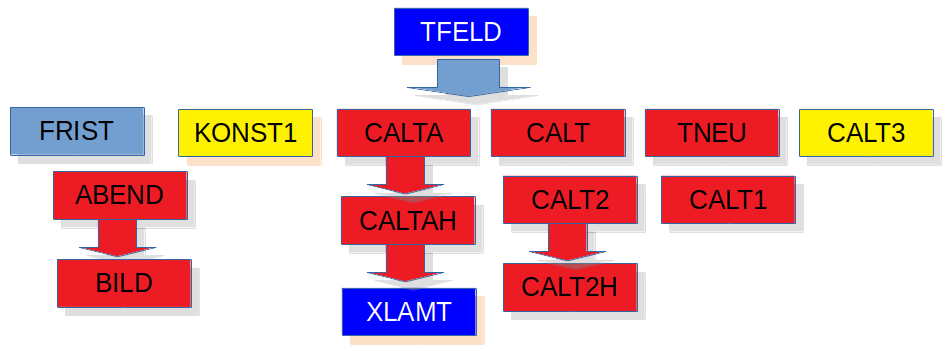
\includegraphics[scale=.5]{../tfeld.png}
    \caption{Sub rutin \texttt{TFELD}}
    \label{fig:tfeld}
  \end{center}
\end{figure}

\begin{figure}[h!]
  \begin{center}
    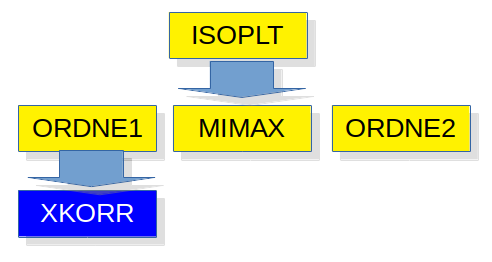
\includegraphics[scale=.5]{../isoplt.png}
    \caption{Sub rutin \texttt{ISOPLT}}
    \label{fig:isoplt}
  \end{center}
\end{figure}

\begin{figure}[h!]
  \begin{center}
    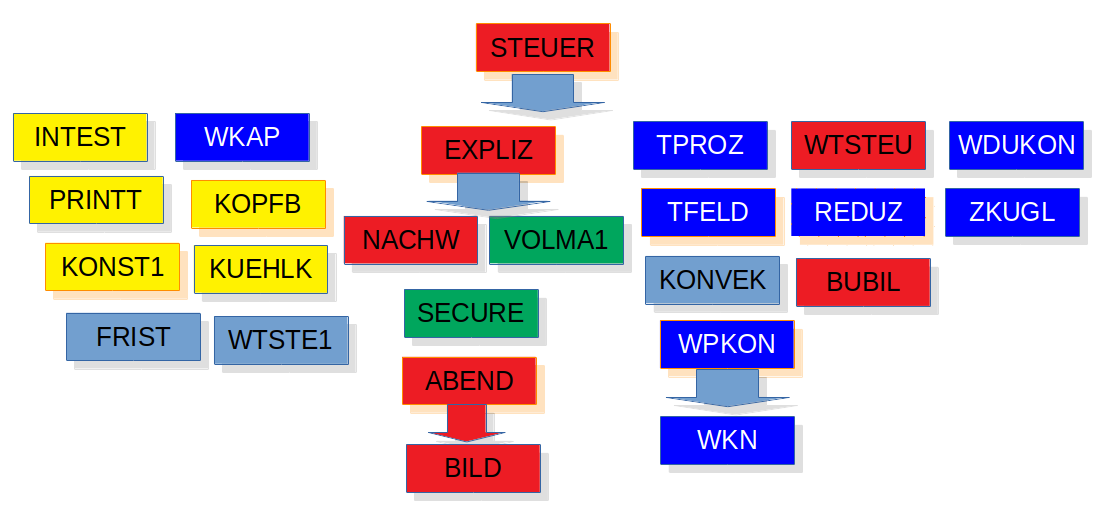
\includegraphics[scale=.5]{../steuer.png}
    \caption{Sub rutin \texttt{STEUER}}
    \label{fig:steuer}
  \end{center}
\end{figure}

Untuk sub rutin \texttt{SETSTR} tidak ditampilkan karena hanya membawahi \texttt{ABEND} yang sudah ditampilkan di \figurename~\ref{fig:maithx}. sedangkan sub rutin \texttt{SETT} bersama sub rutin \texttt{SETF1}, \texttt{SETF2}, \texttt{SETK1} ditampilkan pada \figurename~\ref{fig:varset}. Sub rutin tersebut sama-sama membawahi sub rutin \texttt{ABEND}.

\begin{figure}[h!]
  \begin{center}
    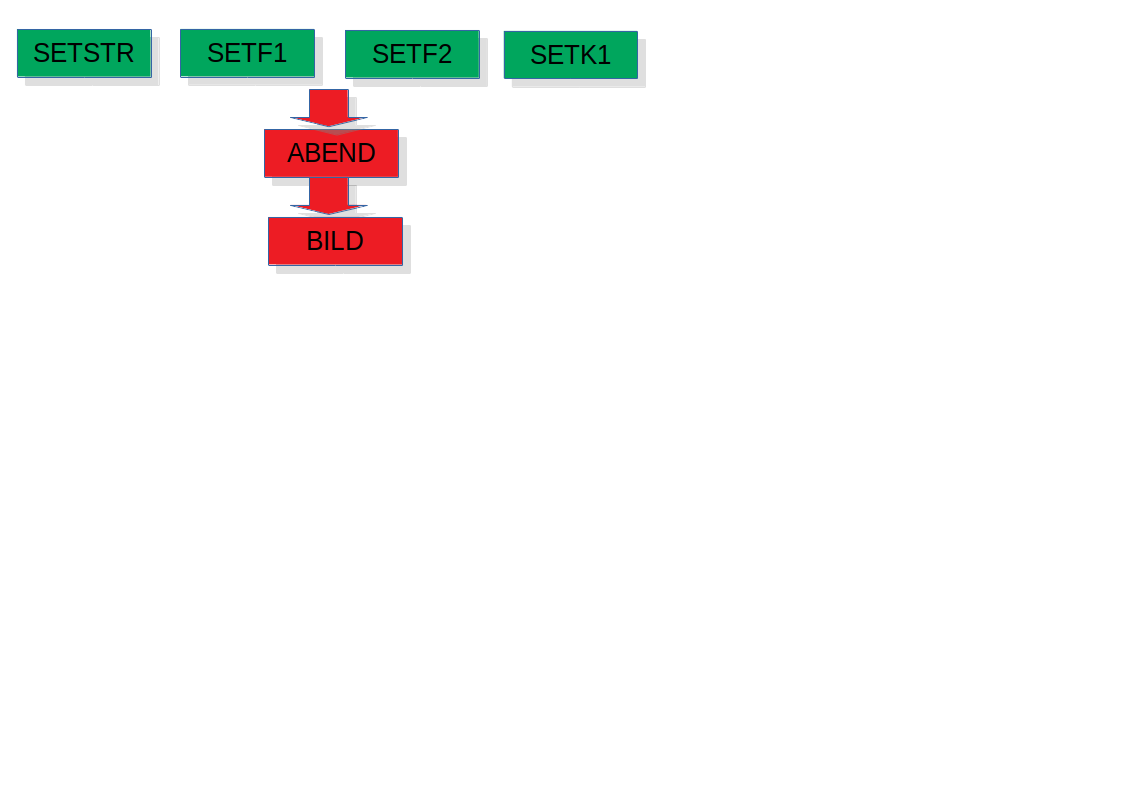
\includegraphics[scale=.5]{../varSET.png}
    \caption{Sub rutin \texttt{VARSET}}
    \label{fig:varset}
  \end{center}
\end{figure}

\section{Diagram alir data level 1}
Diagram yang disajikan pada Gambar \ref{fig:level1} adalah penjabaran dari diagram konteks yang disajikan di Gambar \ref{fig:level0}. Triamix harus menyediakan sub rutin yang dapat menerima informasi rapat daya berikut informasi pendukung berupa dimensi reaktor pada arah radial dan
axial, lengkap dengan jumlah \textit{mesh} pada kedua arah tersebut. Untuk informasi rapat daya, Triamix dirancang untuk dapat membacanya dari berkas teks berisi matriks dua dimensi yang. Jumlah \textit{mesh} di arah radial harus sama dengan jumlah kolom dalam informasi rapat daya. Demikian juga dengan jumlah \textit{mesh} di arah axial, harus sama dengan jumlah baris dalam informasi rapat daya. Sub rutin tersebut dalam Gambar \ref{fig:level1} merupakan sub rutin 1.1, \textit{Input Adapter}. Sedangkan diagram 1.3, \textit{Output Adapter} merupakan sub rutin yang
memformat hasil perhitungan distribusi temperatur sesuai dengan karakterisktik masukan TRIAC-BATAN \cite{triac1}.

\begin{figure}[h!]
  \begin{center}
    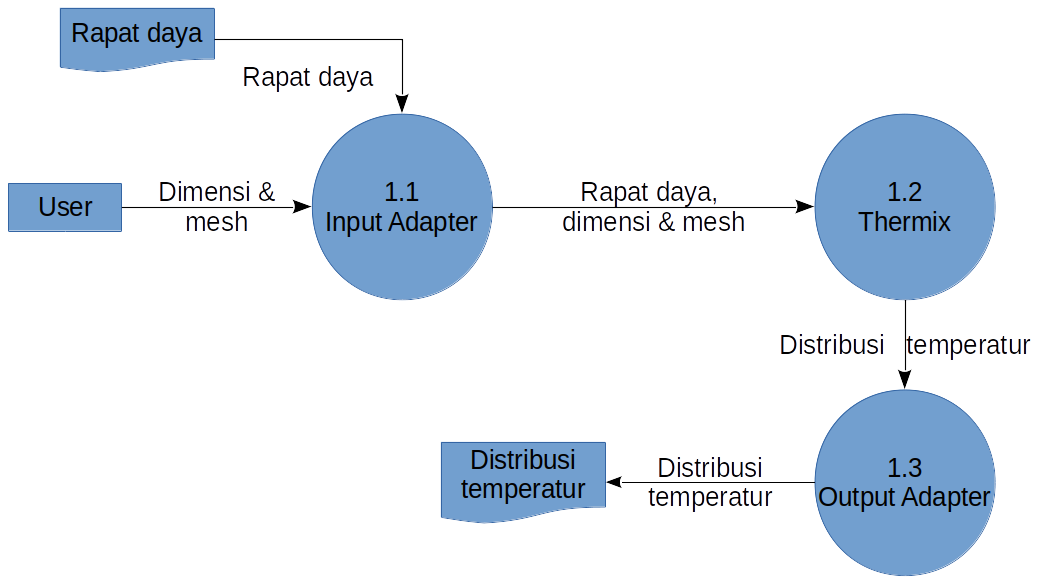
\includegraphics[scale=.5]{pics/level1.png}
    \caption{Diagram alir data level 1}
    \label{fig:level1}
  \end{center}
\end{figure}

Sub rutin perhitungan distribusi temperatur akan dijalankan oleh sub rutin 1.2, \texttt{THERMIX}. Sub rutin tersebut adalah sub rutin \texttt{MAITHX} yang disajikan pada Gambar \ref{fig:maithx}. Sub rutin \texttt{MAITHX} menerima empat argumen, masing-masing adalah N200, NXS, NDR dan KMAT. Selanjutnya, sub rutin STEUER menerima argumen IFKON, ITLAM, TDIFF, NLOOP, IFRED, IFZW, ITM3, CP0, IFTEST, NHET, ZEITH, XFR, IEXPR, N200, NDR, NXS, POV, ZF, NRY, QNW, DELDZ, QTHX, dan WTGINT. Sub rutin \texttt{STEUER} disajikan pada Gambar \ref{fig:steuer}. Terakhir, sub rutin \texttt{TFELD} akan menerima argumen ITLAM, OVRM, IFKO1, IFWARN, CP0, IFZENT. Sub rutin \texttt{TFELD} disajikan pada Gambar \ref{fig:tfeld}.


\chapter{Rancangan Pengujian}
Pengujian yang akan dilakukan pada Triamix adalah white box testing \cite{whitebox,iso}. Pengujian secara white box meliputi:
\begin{itemize}
  \item \textit{Unit testing}: merupakan pengujian unit perangkat keras atau lunak, maupun kelompok unitnya. Dalam hal ini, pengujian hanya akan difokuskan pada pengujian setiap fungsi dan modul.
  \item \textit{Integration testing}: merupakan pengujian terintegrasi antar fungsi dan modul. Validasinya dilakukan terhadap hasil dari berkas masukan yang sama seperti telah dijelaskan dalam dokumen kebutuhan.
\end{itemize}
% Daftar Pustaka
\bibliographystyle{IEEEtran}
\bibliography{references}

%\begin{appendix}
%	\include{markLampiran}
%	\setcounter{page}{2}
%	%-----------------------------------------------------------------------------%
\addChapter{Lampiran 1}
\chapter*{Lampiran 1: Contoh file input}
\label{lamp:inputExample}
%-----------------------------------------------------------------------------%
\includepdf[pages={1-}]{inputExample.pdf}
%\includepdf{inputExample2}

\begin{landscape}
\addChapter{Lampiran 2: InputData.py}
\chapter*{Lampiran 2: InputData.py}
\scriptsize
\lstinputlisting[language=python, numbers=left, numberstyle=\tiny, caption=InputData.py, showstringspaces=false, label=InputData.py]{../Uji/InputData.py}
\normalsize

\addChapter{Lampiran 3: interpolasi.py}
\chapter*{Lampiran 3: interpolasi.py}
\scriptsize
\lstinputlisting[language=python, numbers=left, numberstyle=\tiny, caption=Interpolasi.py, showstringspaces=false, label=Interpolasi.py]{../TRIAC/Interpolasi.py}
\normalsize

\addChapter{Lampiran 4: core.py}
\chapter*{Lampiran 4: core.py}
\scriptsize
\lstinputlisting[language=python, numbers=left, numberstyle=\tiny, caption=core.py, showstringspaces=false, label=core.py]{../Uji/core.py}
\normalsize

\addChapter{Lampiran 5: triac.py}
\chapter*{Lampiran 5: triac.py}
\scriptsize
\lstinputlisting[language=python, numbers=left, numberstyle=\tiny, caption=triac.py, showstringspaces=false, label=triac.py]{../Uji/triacd.py}
\normalsize

\addChapter{Lampiran 6: LHScalculation.py}
\chapter*{Lampiran 6: LHScalculation.py}
\scriptsize
\lstinputlisting[language=python, numbers=left, numberstyle=\tiny, caption=LHScalculation.py, showstringspaces=false, label=LHScalculation.py]{../Uji/LHScalculation.py}
\normalsize

\addChapter{Lampiran 7: lhs.py}
\chapter*{Lampiran 7: lhs.py}
\scriptsize
\lstinputlisting[language=python, numbers=left, numberstyle=\tiny, caption=lhs.py, showstringspaces=false, label=lhs.py]{../Uji/lhs.py}
\normalsize

\addChapter{Lampiran 8: uniform.py}
\chapter*{Lampiran 8: uniform.py}
\scriptsize
\lstinputlisting[language=python, numbers=left, numberstyle=\tiny, caption=uniform.py, showstringspaces=false, label=uniform.py]{../Uji/uniform.py}
\normalsize

\addChapter{Lampiran 9: triangle.py}
\chapter*{Lampiran 9: triangle.py}
\scriptsize
\lstinputlisting[language=python, numbers=left, numberstyle=\tiny, caption=triangle.py, showstringspaces=false, label=triangle.py]{../Uji/triangle.py}
\normalsize

\addChapter{Lampiran 10: normal.py}
\chapter*{Lampiran 10: normal.py}
\scriptsize
\lstinputlisting[language=python, numbers=left, numberstyle=\tiny, caption=normal.py, showstringspaces=false, label=normal.py]{../Uji/normal.py}
\normalsize
\end{landscape}

%\end{appendix}

\end{document}
